\section{Object 8}
\markright{Object 8}

This part was created through a sequence of extrusion and cut operations. The process started with sketching and extruding the main base. Following that, two rectangular profiles were sketched and extruded from the sides. The final step involved using the Extruded Cut feature to create the circular holes, completing the model's geometry.

\begin{figure}[H]
	\centering

	\begin{subfigure}[b]{0.49\textwidth}
		\centering
		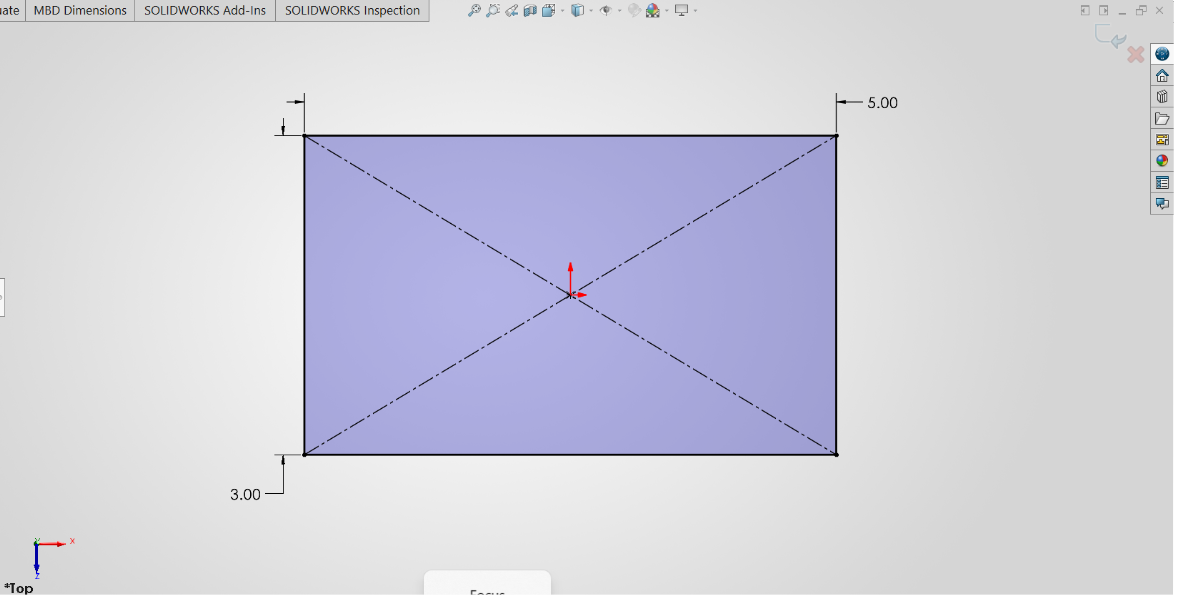
\includegraphics[width=\textwidth, keepaspectratio]{lab-01/assets/object-8/object-8-snap-1.png}
		\caption{2D sketch of the base with dimensions.}
	\end{subfigure}%
	\hfill
	\begin{subfigure}[b]{0.49\textwidth}
		\centering
		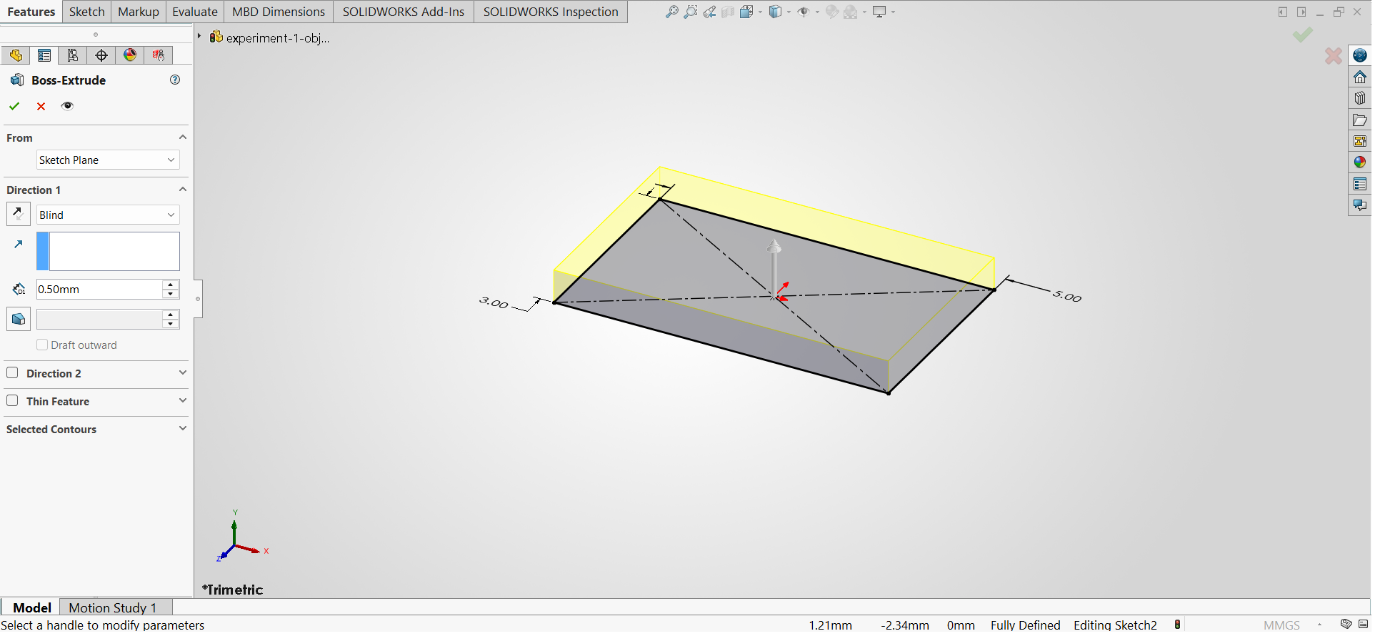
\includegraphics[width=\textwidth, keepaspectratio]{lab-01/assets/object-8/object-8-snap-2.png}
		\caption{Extruding the base.}
	\end{subfigure}%
	\vspace{0.5em}
	\begin{subfigure}[b]{0.49\textwidth}
		\centering
		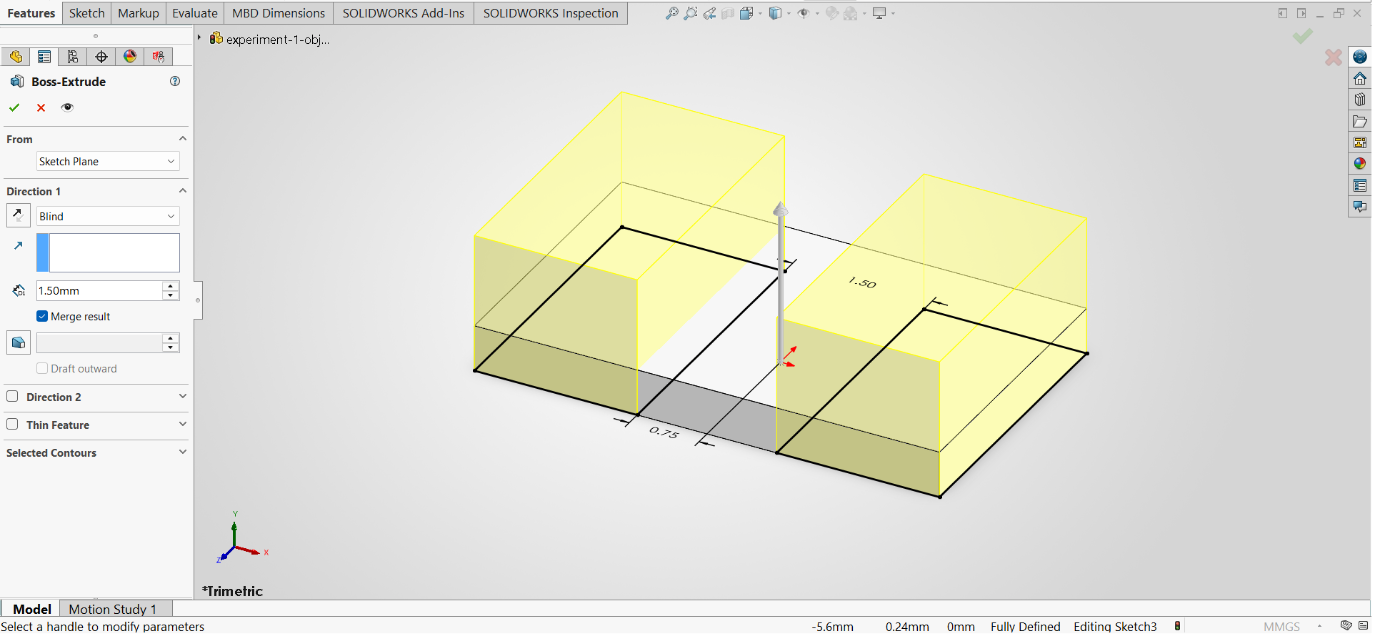
\includegraphics[width=\textwidth, keepaspectratio]{lab-01/assets/object-8/object-8-snap-5.png}
		\caption{Extruding two rectangles from each side.}
	\end{subfigure}%
	\hfill
	\begin{subfigure}[b]{0.49\textwidth}
		\centering
		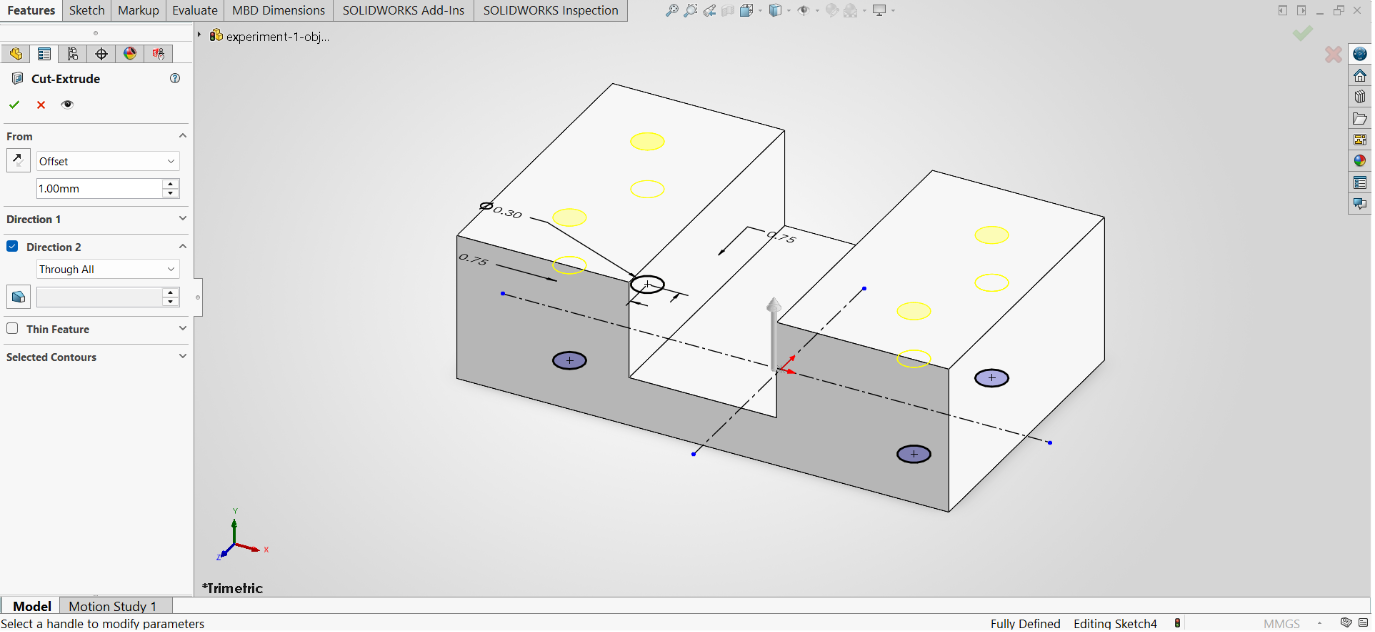
\includegraphics[width=\textwidth, keepaspectratio]{lab-01/assets/object-8/object-8-snap-8.png}
		\caption{Cutting off the holes.}
	\end{subfigure}%
	\vspace{0.5em}
	\begin{subfigure}[b]{\textwidth}
		\centering
		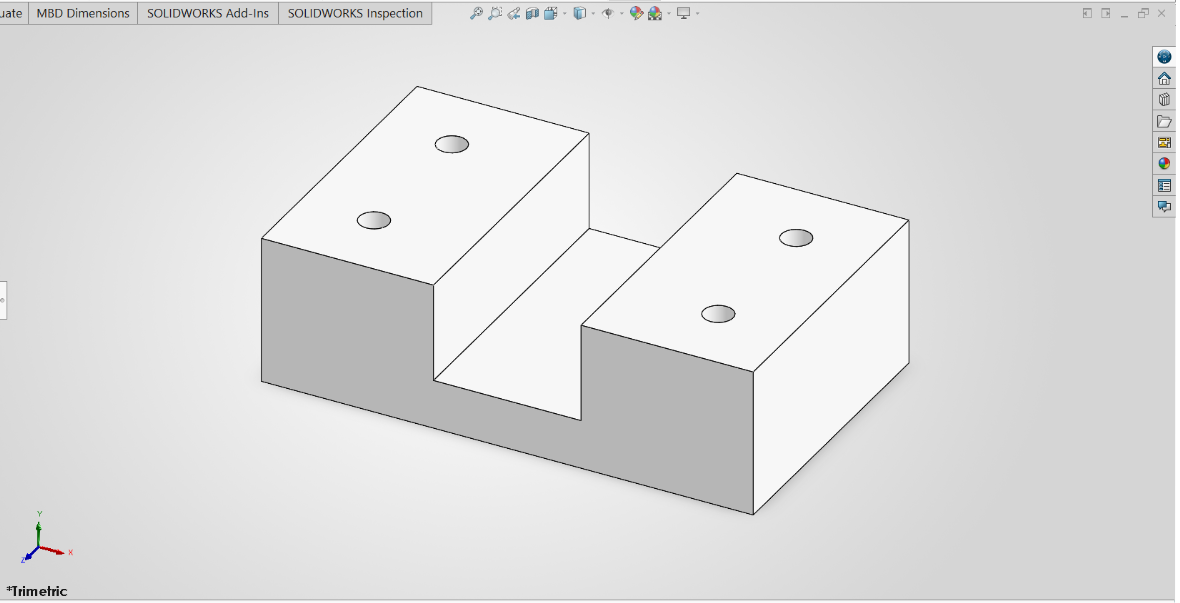
\includegraphics[width=\textwidth, keepaspectratio]{lab-01/assets/object-8/object-8-snap-9.png}
		\caption{Final result.}
	\end{subfigure}

	\caption{Snapshots while Designing Object 8 in Solidworks}
	\label{lab01_object_8}
\end{figure}
